\documentclass[11pt]{article}
\usepackage[utf8]{inputenc}
\usepackage{float}
\usepackage{amsmath}
\usepackage{tikz} % for Hasse diagram
\usepackage[hmargin=3cm,vmargin=6.0cm]{geometry}
%\topmargin=0cm
\topmargin=-2cm
\addtolength{\textheight}{6.5cm}
\addtolength{\textwidth}{2.0cm}
%\setlength{\leftmargin}{-5cm}
\setlength{\oddsidemargin}{0.0cm}
\setlength{\evensidemargin}{0.0cm}

\begin{document}
	
\section*{Student Information } 
%Write your full name and id number between the colon and newline
%Put one empty space character after colon and before newline
Full Name : Yavuz Selim YEŞİLYURT \\
Id Number :  2259166 \\

% Write your answers below the section tags
\section*{Answer 1}
To find largest possible number of vertices in a graph with 23 edges all vertices having degree at least 4 we can use the \textbf{handshaking theorem}. Handshaking theorem states that:\\
Let G = (V , E) be an undirected graph with m edges. Then\\\\
$2m=\sum\limits_{v \in V} degv$\\\\
We have 23 edges in our graph, since we want to find the \textbf{largest} possible number of vertices we should consider the cases when each vertices in the graph have the least possible degree, namely 4. Therefore our problem turns into:\\\\
\begin{equation*}
\begin{split}
2E	 &=  deg(v_1) + deg(v_2) +...+ deg(v_n)   \\
2.23	 &=  4 + 4 +...+ 2 \\
46	 &=  4.11 + 2  \qquad \qquad \ \ \	(1)\\
\end{split}	 
\end{equation*} \\ 
Hence from (1) we can say there are at most 11 possible such vertices having degree at least 4 (One can say this graph contains 10 vertices with degree 4 and 1 vertice with degree 6 or 9 vertices with degree 4 and 2 vertices with degree 5)\\

\section*{Answer 2}
In our problem we have a graph $G$ with n vertices each of which has degree $d \geq \frac{n-1}{2}$.\\

If $G$ has $n = 2$ vertices then we can say there is a hamiltonian path in $G$. Each vertice has degree $d \geq \frac{2-1}{2} =\frac{1}{2}$, namely each of the two vertices have degree 1. We can show the existance of Hamiltonian path with going from one vertice to another and stop there with saying that it's a Hamiltonian path.\\

If $G$ has $n\geq 3$ vertices, we can utilize the \textbf{Dirac's Theorem}. Dirac's Theorem states that:\\
If $G$ is a simple graph with $n$ vertices with $n\geq 3$ such that the degree of every vertex in $G$ is at least $\frac{n}{2}$, then $G$ has a Hamiltonian circuit.\\

Consider a new graph $R$ which is the same graph as $G$ except it has a new vertice $v$ in addition to $G$'s vertices and say this new vertice $v$ is connected to all other vertices in the graph, therefore it contributes $+1$ to the degrees of each vertice in the graph $R$. So we have:\\

$\frac{n-1}{2} + 1 = \frac{n+1}{2}$\\\\ Which means our new graph $R$ has $n+1$ vertices, each of which has degree $d \geq \frac{n+1}{2}$. We can clearly see that graph $R$ obeys Dirac's Theorem (because $\frac{n+1}{2} > \frac{n}{2}$) , namely it has a Hamiltonian circuit.\\\\
Now we can remove the additional vertice $v$ on $R$ and get again $G$, which will imply that the Hamiltonian circuit on $R$ is broken but since we remove 1 vertice the remaining part will construct a Hamiltonian path with $n$ vertices, each of which has degree $d \geq \frac{n-1}{2}$. Therefore we can say $G$ contains a Hamiltonian path.\\

\section*{Answer 3}
We know a simple graph $G$ is called \textbf{bipartite} if its vertice set $V$ can be partitioned into two disjoint sets $V_1$ and $V_2$ such that every edge in the graph connects a vertex in $V_1$ and a vertex in $V_2$ (so that no edge in G connects either two vertices in $V_1$ or two vertices in $V_2$ and hence there can not be any loops inside any of the sets $V_1$ and $V_2$) and we know that in adjacency matrix representation of $G$ we have the following rule:\\\\
$a_{ij} = 1$ if \{$v_i,v_j$\} is an edge of $G$\\
$a_{ij} = 0$ otherwise\\

Now let our bipartite graph be $G$ with adjacency matrix $A$. We can easily conclude from the rule of adjacency matrix above, that diagonal entries of $A$ are equal to $0$ if and only if each vertice in our graph $G$ does not have any loops (i.e. edge to itself). Since our graph is bipartite, as we stated above, it can not have any loops inside. So it means that diagonal entries of $A^1$ are equal to $0$. Now for $A^{37}$ we check the following powers of $A$ and we see that for even powers of $A$ we have the reverse diagonal entries which are equal to $0$ and for odd powers of $A$ we have the diagonal entries which are equal to $0$. Since 37 is odd, we can say diagonal entries of $A^{37}$ are equal to $0$.\\

\section*{Answer 4}
\begin{itemize}
	\item[\textbf{a.}] 
	Let's write the pseudocode of the \textbf{Kruskal's Algorithm};\\
	1. Sort all the edges in non-decreasing order of their weight.\\
	2. Pick the smallest edge (in terms of their weight). Check if it forms a simple circuit with the spanning tree formed so far. If circuit is not formed, include this edge. Else, discard it.\\
	3. Repeat step 2 until there are $(V-1)$ edges in the spanning tree.\\
\newpage
	Start with step 1, order the edges of our graph in non-decreasing order of their weight on a Choice-Edge-Weight table:\\
	\begin{table}[H]
	\small
	\centering
	\begin{tabular}{|c|c|c|}	
	\hline
	$Choice$ & $Edge$ & $Weight$\\
	\hline 
	1 & $\{e,f\}$ & 1\\			
	2 & $\{e,h\}$ & 2\\	
	3 & $\{g,h\}$ & 2\\	
	4 & $\{a,d\}$ & 2\\	
	5 & $\{d,g\}$ & 3 \\	
	6 & $\{d,b\}$ & 3 \\	
	7 & $\{h,f\}$ & 3 \\	
	8 & $\{c,f\}$ & 3 \\	
	9 & $\{b,c\}$ & 4 \\	
	10& $\{h,i\}$ & 4 \\	
	11& $\{a,b\}$ & 5 \\	
	12& $\{b,e\}$ & 5 \\	
	13& $\{f,i\}$ & 5 \\	
	14& $\{b,f\}$ & 6 \\	
	15& $\{d,e\}$ & 7 \\
	16& $\{d,h\}$ & 8 \\
	\hline 
	\end{tabular}
	\end{table}
	Go on with step 2, Smallest edge is \{e,f\} no circuit is formed so we pick it. There aren't $(V-1)$ edges in the spanning tree so we repeat step 2, next smallest edges \{e,h\},\{g,h\} and \{a,d\}, each have same weight, namely 2 and neither of them forms a circuit with the spanning tree formed so far, so we pick all of them. There aren't $(V-1)$ edges in the spanning tree so we repeat step 2, next smallest edges \{d,g\},\{d,b\},\{h,f\} and \{c,f\} each have same weight, namely 3.  \{d,g\},\{d,b\} and \{c,f\} does not form a circuit with the spanning tree formed so far, but \{h,f\} forms a circuit in the spanning tree, so we just pick \{d,g\},\{d,b\} and \{c,f\} and discard \{h,f\}. There aren't $(V-1)$ edges in the spanning tree so we repeat step 2, next smallest edges \{b,c\} and \{h,i\} each have same weight, namely 4. \{h,i\} does not form a circuit with the spanning tree formed so far, but \{b,c\} forms a circuit in the spanning tree, so we just pick \{h,i\} and discard \{b,c\}. There are $(V-1)$ edges in the spanning tree so we stop here. The minimum spanning tree we obtained is:\\

\begin{figure}[H]	\caption{MST acquired with Kruskal's algorithm for the given graph}
	\centering
	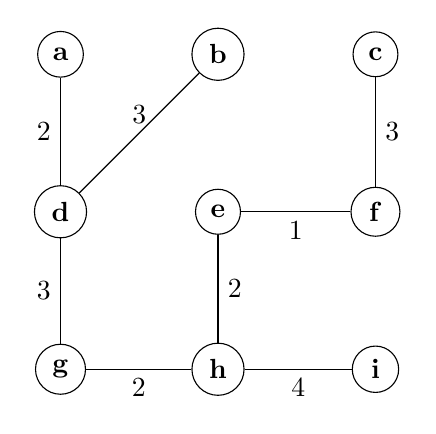
\begin{tikzpicture}
	
	\node[shape=circle,draw=black] (a) at (0, 4)     {\textbf{a}};
	\node[shape=circle,draw=black] (b) at (2, 4)     {\textbf{b}};
	\node[shape=circle,draw=black] (c) at (4, 4)     {\textbf{c}};
	\node[shape=circle,draw=black] (d) at (0, 2)     {\textbf{d}};
	\node[shape=circle,draw=black] (e) at (2, 2)     {\textbf{e}};
	\node[shape=circle,draw=black] (f) at (4, 2)     {\textbf{f}};
	\node[shape=circle,draw=black] (g) at (0, 0)     {\textbf{g}};
	\node[shape=circle,draw=black] (h) at (2, 0)     {\textbf{h}};
	\node[shape=circle,draw=black] (i) at (4, 0)     {\textbf{i}};
	
	\path[-] (a) edge  node[left]  {2} (d);
	\path[-] (b) edge  node[above] {3} (d);
	\path[-] (c) edge  node[right] {3} (f);
	\path[-] (d) edge  node[left]  {3} (g);
	\path[-] (e) edge  node[right] {2} (h);
	\path[-] (e) edge  node[below] {1} (f);
	\path[-] (g) edge  node[below] {2} (h);
	\path[-] (h) edge  node[below] {4} (i);
	
	\end{tikzpicture} 
\end{figure}
\newpage
	\item[\textbf{b.}] \end{itemize}
	Let's write the pseudocode of the \textbf{Prim's Algorithm};\\
	1. Initialize the minimum spanning tree with a vertice chosen at random.\\
	2. Find all the edges that connect the tree to new vertices, find the minimum and add it to the tree.\\
	3. Repeat step 2 until there are $(V-1)$ edges in the spanning tree.\\

	We will write choices on each step Choice-Edge-Weight table.\\
	\begin{table}[H]
	\small
	\centering
	\begin{tabular}{|c|c|c|}	
	\hline
	$Choice$ & $Edge$ & $Weight$\\
	\hline 
	1 & $\{a,d\}$ & 2\\			
	2 & $\{d,b\}$ & 3\\	
	3 & $\{d,g\}$ & 3\\
	4 & $\{g,h\}$ & 2\\
	5 & $\{h,e\}$ & 2\\	
	6 & $\{e,f\}$ & 1\\
	7 & $\{f,c\}$ & 3\\
	8 & $\{h,i\}$ & 4\\	
	\hline 
	\end{tabular}
	\end{table}
	Start with step 1, initialize the minimum spanning tree with a vertice \{a\} (chosen randomly). Go on with step 2, the minimum edge that connects tree to new vertices is \{a,d\} with weight 2, so we pick it. There aren't $(V-1)$ edges in the spanning tree so we repeat step 2, the minimum edge that connects tree to new vertices is \{d,b\} with weight 3, so we pick it. There aren't $(V-1)$ edges in the spanning tree so we repeat step 2, the minimum edge that connects tree to new vertices is \{d,g\} with weight 3, so we pick it. There aren't $(V-1)$ edges in the spanning tree so we repeat step 2, the minimum edge that connects tree to new vertices is \{g,h\} with weight 2, so we pick it. There aren't $(V-1)$ edges in the spanning tree so we repeat step 2, the minimum edge that connects tree to new vertices is \{h,e\} with weight 2, so we pick it. There aren't $(V-1)$ edges in the spanning tree so we repeat step 2, the minimum edge that connects tree to new vertices is \{e,f\} with weight 1, so we pick it. There aren't $(V-1)$ edges in the spanning tree so we repeat step 2, the minimum edge that connects tree to new vertices is \{f,c\} with weight 3, so we pick it. There aren't $(V-1)$ edges in the spanning tree so we repeat step 2, the minimum edge that connects tree to new vertices is \{h,i\} with weight 4, so we pick it. There are $(V-1)$ edges in the spanning tree so we stop here. The minimum spanning tree we obtained is:\\

\begin{figure}[H]	\caption{MST acquired with Prim's algorithm for the given graph}
	\centering
	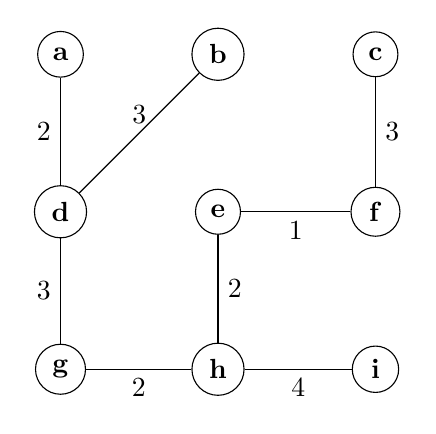
\begin{tikzpicture}
	
	\node[shape=circle,draw=black] (a) at (0, 4)     {\textbf{a}};
	\node[shape=circle,draw=black] (b) at (2, 4)     {\textbf{b}};
	\node[shape=circle,draw=black] (c) at (4, 4)     {\textbf{c}};
	\node[shape=circle,draw=black] (d) at (0, 2)     {\textbf{d}};
	\node[shape=circle,draw=black] (e) at (2, 2)     {\textbf{e}};
	\node[shape=circle,draw=black] (f) at (4, 2)     {\textbf{f}};
	\node[shape=circle,draw=black] (g) at (0, 0)     {\textbf{g}};
	\node[shape=circle,draw=black] (h) at (2, 0)     {\textbf{h}};
	\node[shape=circle,draw=black] (i) at (4, 0)     {\textbf{i}};
	
	\path[-] (a) edge  node[left]  {2} (d);
	\path[-] (b) edge  node[above] {3} (d);
	\path[-] (c) edge  node[right] {3} (f);
	\path[-] (d) edge  node[left]  {3} (g);
	\path[-] (e) edge  node[right] {2} (h);
	\path[-] (e) edge  node[below] {1} (f);
	\path[-] (g) edge  node[below] {2} (h);
	\path[-] (h) edge  node[below] {4} (i);
	
	\end{tikzpicture} 
\end{figure}

\end{document}